\documentclass{standalone}
\usepackage{graphicx}	
\usepackage{amssymb, amsmath}
\usepackage{color}

\usepackage{tikz}
\usetikzlibrary{intersections, backgrounds}
\usepackage{pgfmath}

\definecolor{light}{RGB}{220, 188, 188}
\definecolor{mid}{RGB}{185, 124, 124}
\definecolor{dark}{RGB}{143, 39, 39}
\definecolor{highlight}{RGB}{180, 31, 180}
\definecolor{gray10}{gray}{0.1}
\definecolor{gray20}{gray}{0.2}
\definecolor{gray30}{gray}{0.3}
\definecolor{gray40}{gray}{0.4}
\definecolor{gray60}{gray}{0.6}
\definecolor{gray70}{gray}{0.7}
\definecolor{gray80}{gray}{0.8}
\definecolor{gray90}{gray}{0.9}
\definecolor{gray95}{gray}{0.95}

\begin{document}

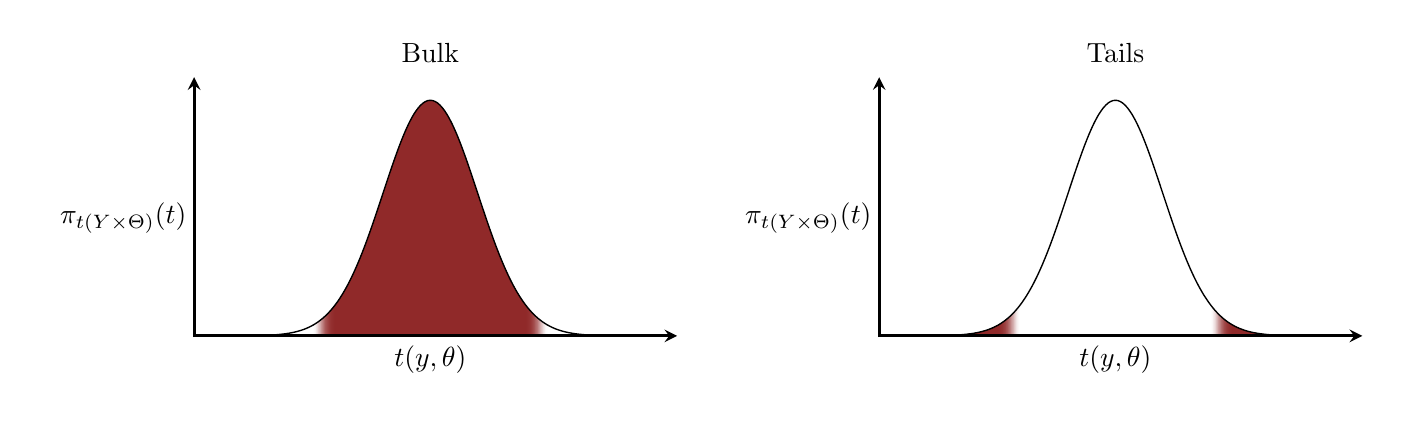
\begin{tikzpicture}[scale=0.3, thick,
declare function={ g(\x) = exp(-0.5 * (\x - 0) * (\x - 0) / (2 * 2)) / (2.506628274631001 * 2);}
]

  \pgfmathsetmacro{\dx}{0}
  
  \draw[color=white] (-17 + \dx, -2.5) rectangle (12 + \dx, 13);
   
  \foreach \i in {0, 0.05, ..., 1} {
    \begin{scope}
    \clip ({-5 + \i}, 0) rectangle ({5 - \i}, 10);
    \pgfmathsetmacro{\prop}{100 * exp(-5.0 * \i * \i)};
    \colorlet{custom}{white!\prop!dark};
    \fill[color=custom, domain=-10:10, smooth, samples=100, variable=\x] 
      plot ({\x}, {50 * g(\x)});
    \end{scope}
  }

  \draw[color=black, domain=-10:10, smooth, samples=100, variable=\x, line width=0.5] 
    plot ({\x}, {50 * g(\x)});

  \node[] at (-13, 5) { $\pi_{t(Y \times \Theta)} (t)$ };

  \draw [->, >=stealth, line width=1] (-10.05, 0) -- +(20.5, 0);
  \draw [->, >=stealth, line width=1] (-10, -0.05) -- +(0, 11);
  \node[] at (0, -1) { $t(y, \theta)$ };
  
  \node[] at (0, 12) { Bulk };
   
  \pgfmathsetmacro{\dx}{29}
  
  \draw[color=white] (-17 + \dx, -2.5) rectangle (12 + \dx, 13);
   
  \foreach \i in {0, 0.05, ..., 1} {
    \begin{scope}
    \clip (-10 + \dx, 0) rectangle ({-4 - \i + \dx}, 10);
    \pgfmathsetmacro{\prop}{100 * exp(-5.0 * \i * \i)};
    \colorlet{custom}{white!\prop!dark};
    \fill[color=custom, domain=-10:10, smooth, samples=100, variable=\x] 
      plot ({\x + \dx}, {50 * g(\x)});
    \end{scope}
    
    \begin{scope}
    \clip ({4 + \i + \dx}, 0) rectangle (10 + \dx, 10);
    \pgfmathsetmacro{\prop}{100 * exp(-5.0 * \i * \i)};
    \colorlet{custom}{white!\prop!dark};
    \fill[color=custom, domain=-10:10, smooth, samples=100, variable=\x] 
      plot ({\x + \dx}, {50 * g(\x)});
    \end{scope}
  }
  
  \draw[color=black, domain=-10:10, smooth, samples=100, variable=\x, line width=0.5] 
    plot ({\x + \dx}, {50 * g(\x)});

  \node[] at (-13 + \dx, 5) { $\pi_{t(Y \times \Theta)} (t)$ };

  \draw [->, >=stealth, line width=1] (-10.05 + \dx, 0) -- +(20.5, 0);
  \draw [->, >=stealth, line width=1] (-10 + \dx, -0.05) -- +(0, 11);
  \node[] at (0 + \dx, -1) { $t(y, \theta)$ };
  
  \node[] at (0 + \dx, 12) { Tails };
  
\end{tikzpicture}

\end{document}  